%%%%%%%%%%%%%%%%%%%%%%%%%%%%%%%%%%%%%%%%%%%%%%%%%%%%%%%%%%%%%%%%%%%%%%%%%%%%%%%%
%                                                                              %
%   HIGZ  User Guide -- LaTeX Source                                           %
%                                                                              %
%   Chapter: Graphics macroprimitives                                          %
%                                                                              %
%   This document needs the following external EPS files:                      %
%            box.eps                                                           %
%            fbox.eps                                                          %
%            pave.eps                                                          %
%            arc.eps                                                           %
%            graph.eps                                                         %
%            hist.eps                                                          %
%            scatter.eps                                                       %
%            boxes.eps                                                         %
%            arrows.eps                                                        %
%            contour.eps                                                       %
%            colour.eps                                                        %
%            tabt.eps                                                          %
%            tabk.eps                                                          %
%            lego.eps                                                          %
%            lego1.eps                                                         %
%            lego2.eps                                                         %
%            surf.eps                                                          %
%            surf1.eps                                                         %
%            surf2.eps                                                         %
%            surf3.eps                                                         %
%            surf4.eps                                                         %
%            surfpol.eps                                                       %
%            surfcyl.eps                                                       %
%            surfsph.eps                                                       %
%            surfpsd.eps                                                       %
%            pie.eps                                                           %
%            higzaxis.eps                                                      %
%            softtext.eps                                                      %
%                                                                              %
%   Editor: Olivier Couet / CN-AS                                              %
%   Last Mod.: 9 July 1993 oc                                                  %
%                                                                              %
%%%%%%%%%%%%%%%%%%%%%%%%%%%%%%%%%%%%%%%%%%%%%%%%%%%%%%%%%%%%%%%%%%%%%%%%%%%%%%%%
\Filename{H1Thegraphicmacroprimitives}
\chapter{The graphic macroprimitives}
\index{graphic!macroprimitives}

In addition to the standard set of basic graphic primitives describe
in the previous chapter, \HIGZ~provides also a set of graphic "macroprimitives".
\index{macroprimitive} 
These graphic macroprimitives are included in \HIGZ~for three main reasons:
\begin{enumerate}
\item Functionality: it is easier to define a circle with its center and its
      radius than to compute all the necessary points to draw a polyline.
\item Precision, for instance a circle has to be stored as a circle and not as
      a sequence of polylines.
\item Compactness of the graphic data base.
\index{picture!data base}
\end{enumerate}
 
\Filename{H2Drawingabox}
\section{Drawing a box}
\index{box!drawing}
\Shubr{IGBOX}{(X1,X2,Y1,Y2)}
\Action
This routine fills a rectangle according to the ``fill area colour index''
(see section \ref{ISFACI}), the ``fill area interior style'' (see section
\ref{ISFAIS}), and the ``fill area style index'' (see section \ref{ISFASI})
attributes. The border is never drawn unless the interior
style is hollow or the routine \Rind{IGSET} has been called with '\Sind{BORD}'
and {\tt VAL = 1.}. As it is shown on the figure \ref{BOX}, the border of the
rectangle is drawn according to the values of the ``line width scale factor''
(see section \ref{ISLWSC}) and the ``polyline colour index'' (see section
\ref{ISPLCI}) attributes, whereas the ``line type'' is always solid (see
section \ref{ISLN}).
\Pdesc
\begin{DLtt}{123}
\item[X1] X coordinate of 1st corner of the rectangle in \wc.
\item[X2] X coordinate of 2nd corner of the rectangle in \wc.
\item[Y1] Y coordinate of 1st corner of the rectangle in \wc.
\item[Y2] Y coordinate of 2nd corner of the rectangle in \wc.
\end{DLtt}

\begin{Fighere}
\begin{center}\mbox{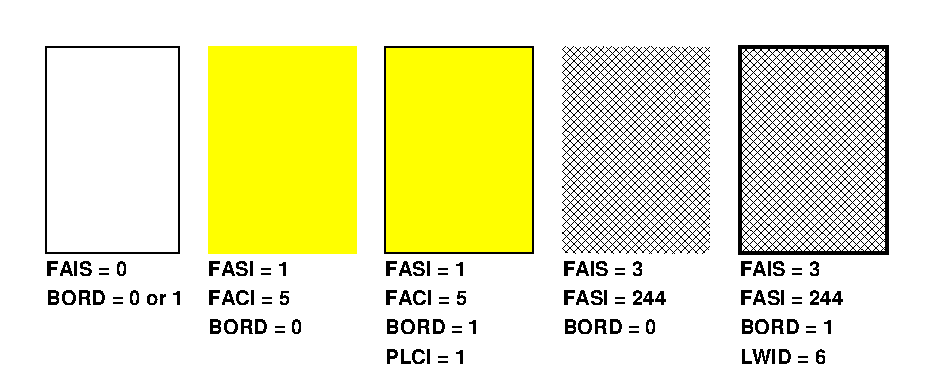
\epsfig{file=box.eps}}\end{center}
\caption{Action of the fill area and polyline attributes on 
\protect\Rind{IGBOX}.}
\label{BOX}
\end{Fighere}
 
\vfill\newpage
\Filename{H2Drawingaframe}
\section{Drawing a frame}
\index{frame!drawing}
\Shubr{IGFBOX}{(X1,X2,Y1,Y2,X3,X4,Y3,Y4)}
\Action
This routine fills a frame according to the ``fill area colour index''
(see section \ref{ISFACI}), the ``fill area interior style'' (see section
\ref{ISFAIS}), and the ``fill area style index'' (see section \ref{ISFASI})
attributes. The border is never drawn unless the interior
style is hollow or the routine \Rind{IGSET} has been called with '\Sind{BORD}'
and {\tt VAL = 1.}. Like for the \Rind{IGBOX} primitive (see figure \ref{BOX}),
the border of the frame is drawn according to the values of the ``line width
scale factor'' (see section \ref{ISLWSC}) and the ``polyline colour index''
(see section \ref{ISPLCI}) attributes, whereas the ``line type'' is always solid
(see section \ref{ISLN}).
\Pdesc
\begin{DLtt}{123}
\item[X1] X coordinate of 1st corner of the outer rectangle in \wc.
\item[X2] X coordinate of 2nd corner of the outer rectangle in \wc.
\item[Y1] Y coordinate of 1st corner of the outer rectangle in \wc.
\item[Y2] Y coordinate of 2nd corner of the outer rectangle in \wc.
\item[X3] X coordinate of 1st corner of the inner rectangle in \wc.
\item[X4] X coordinate of 2nd corner of the inner rectangle in \wc.
\item[Y3] Y coordinate of 1st corner of the inner rectangle in \wc.
\item[Y4] Y coordinate of 2nd corner of the inner rectangle in \wc.
\end{DLtt}
The figure \ref{FBOX} describes the usage of the \Rind{IGFBOX} parameters.

\begin{Fighere}
\begin{center}\mbox{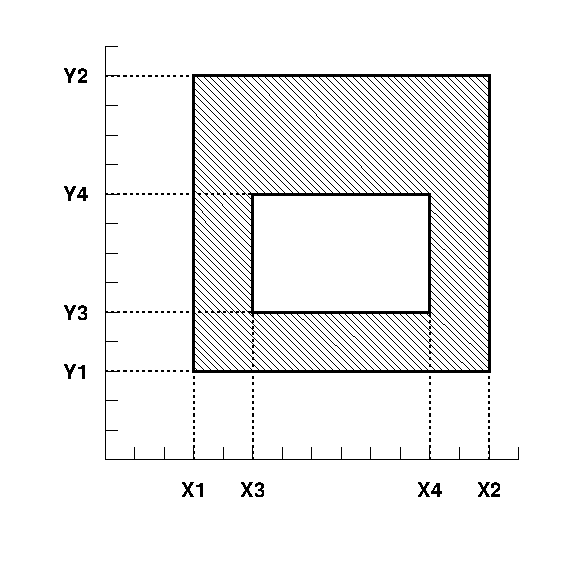
\epsfig{file=fbox.eps}}\end{center}
\caption{Example of \protect\Rind{IGFBOX} usage}
\label{FBOX}
\end{Fighere}
 
\vfill\newpage
\Filename{H2Drawingapavingblock}
\section{Drawing a paving block}
\index{paving block!drawing}
\Shubr{IGPAVE}{(X1,X2,Y1,Y2,DZ,ISBOX,ISFRAM,CHOPT)}
\Action
 This routine draws a paving-block according to the value of {\tt CHOPT}.
 {\tt ISBOX (ISFRAM)} may be {\tt 1000+ICOLOR} where {\tt ICOLOR} is the
colour index of the box (frame), or {\tt 2000+IPAT} where {\tt IPAT} is
the pattern index of the box (frame), otherwise the style index.
If {\tt ISBOX(ISFRAM)=0}, only the box contour is drawn with the current
polyline attributes. By default the Top and the Right frames are drawn.
{\tt CHOPT='TR'}.
\Pdesc
\begin{DLtt}{1234567}
\item[X1]     X bottom left corner of box.
\item[X2]     X top right corner of box.
\item[Y1]     Y bottom left corner of box.
\item[Y2]     Y top right corner of box.
\item[DZ]     Box width.
\item[ISBOX]  Box style.
\item[ISFRAM] Frame style.
\item[CHOPT]  Character option.
\begin{DLtt}{12345}
   \item['T'] The top of the frame is drawn.
   \item['B'] The bottom of the frame is drawn.
   \item['R'] The right part of the frame is drawn.
   \item['L'] The left part of the frame is drawn.
   \item['-'] Reverse sense for the shadow drawing (see figure~\ref{PAVE}).
   \item['S'] The frame is drawn like the ``Shadow'' of the inside box.
   \item['P'] Cut the top of the shadow (see figure~\ref{PAVE}).
   \item['K'] The paving-block is drawn like a button (see figure~\ref{PAVE}).
   \item['D'] Delete. The paving block is drawn in the background colour.
\end{DLtt}
\end{DLtt}
\newpage

\begin{Fighere}
\begin{center}\mbox{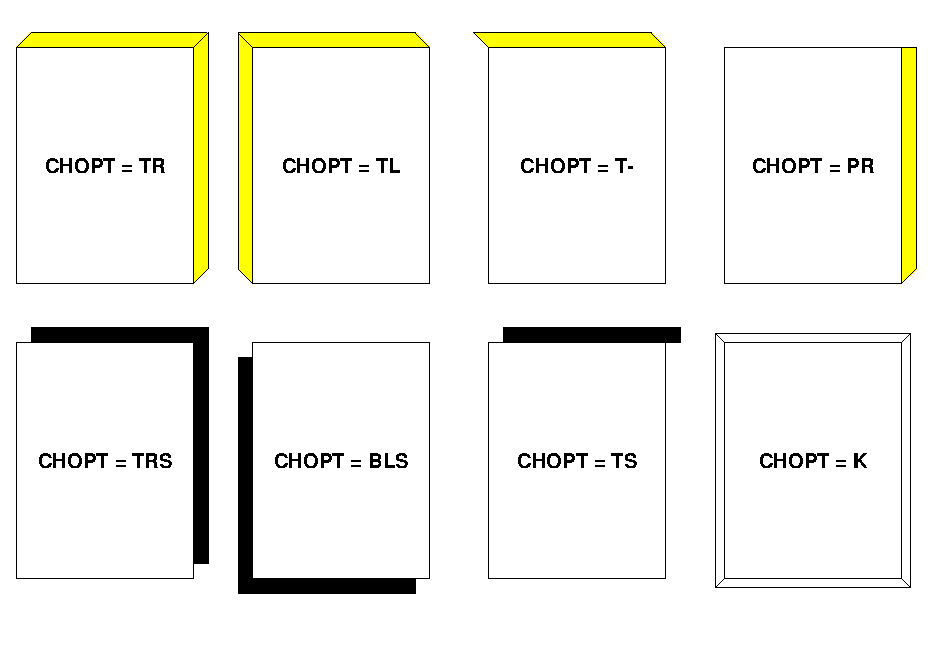
\epsfig{file=pave.eps}}\end{center}
\caption{Examples of \protect\Rind{IGPAVE} usage}
\label{PAVE}
\end{Fighere}
 
\newpage
\Filename{H2Drawinganarc}
\section{Drawing an arc}
\index{arc drawing}
\Shubr{IGARC}{(XC,YC,R1,R2,PHIMIN,PHIMAX)}
\Action
This routine draws one or two arcs of a circle. If the two radii are not equal the area
between the two arcs is filled according to the fill area interior style index
and the fill area style index. The border is never drawn unless the interior
style is hollow or the routine \Rind{IGSET} has been called with \Sind{BORD} and
{\tt VAL = 1}. If the arc's radii are equal only one arc is drawn.
\Pdesc
\begin{DLtt}{1234567}
\item[XC]     X coordinate of the arc's center in world coordinate space.
\item[YC]     Y coordinate of the arc's center in world coordinate space.
\item[R1]     Radius of first arc.
\item[R2]     Radius of second arc.
\item[PHIMIN] Starting angle (degrees.)
\item[PHIMAX] Final angle (degrees.)
\end{DLtt}

\begin{Fighere}
\begin{center}\mbox{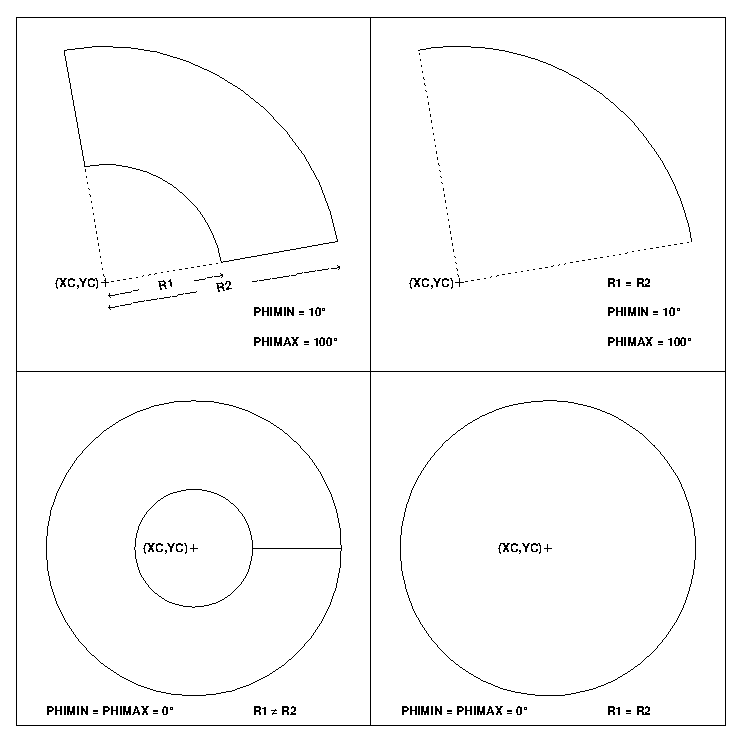
\epsfig{file=arc.eps,height=12cm}}\end{center}
\caption{Examples of \protect\Rind{IGARC}}
\label{fig-FIGU005S}
\end{Fighere}
\vfill
\newpage
\Filename{H2Drawingagraph}
\section{Drawing a graph}
\index{graph drawing}
\Shubr{IGRAPH}{(N,X,Y,CHOPT)}
\Action
This routine draws (in the current \NT) a graph with several possible 
presentations.
\index{curve drawing}
\Pdesc
\begin{DLtt}{1234567}
\item[N]     Number of components in the arrays {\tt X} and {\tt Y}.
\item[X]     Array of dimension {\tt N} containing the x coordinates in
             \WC~space of the graph to be drawn.
\item[Y]     Array of dimension {\tt N} containing the y coordinates in
             \WC~space of the graph to be drawn.
\item[CHOPT] {\tt CHARACTER} variable specifying the options chosen (multiple
             simultaneous options are possible).
\begin{DLtt}{12345}
   \item['R'] The graph is Rotated, i.e. the values in {\tt X} are used
              for the ordinate and the values in {\tt Y} for the abscissa
              (default is the contrary).
   \item['L'] All points are connected with a straight line. (default)
   \item['F'] A Fill area is drawn through the points with the current fill area
              attributes. The border is never drawn unless the fill area 
              interior style is hollow or the routine \Rind{IGSET} has been 
              called with '\Sind{BORD}' and {\tt VAL = 1.}.
   \item['C'] The values in {\tt Y} are plotted in the form of a smooth curve.
              Spline approximation algorithms are used. This option can be used
              with option F in order to draw a smooth fill area.
   \item['*'] A star is plotted at every point.
   \item['P'] A marker is plotted at every point, according to the current
              polymarker attributes.
   \item['B'] The values in {\tt Y} are plotted in the form of bars.
              The width of the bar is by default 50\% of the interval
              {\tt X(I)-X(I-1)}. This percentage can be changed by calling
              \Rind{IGSET} with option \Sind{BARW}.
   \item['A'] X and Y axes are drawn on the border of the current \NT.
   \item['GX'] Logarithmic scale on the X axis.
   \item['GY'] Logarithmic scale on the Y axis.
\end{DLtt}
\end{DLtt}

\newpage
\begin{XMPt}{Example of {\tt GRAPH} drawing (see result on figure \ref{GRAPH})}
      program  graph 
      character*4 chopt(4)
      dimension x(9),y(9)
      parameter (xsize=16.,ysize=20.)
      data x/0.,.6,.3,.2,-.3,.3,-.2,-.3,-.6/
      data y/0.,-.2,-.7,-.9,-.2,.2,.9,.7,.2/
      data chopt/'AL*','AC*','AF*','ACF*'/
*
      call start('graph',xsize,ysize)
*
*              Viewports definition
*
      xnorm  = min(1.,xsize/ysize)
      xnorm2 = xnorm/2.
      ynorm  = min(1.,ysize/xsize)
      ynorm2 = ynorm/2.
      rmarg  = 0.05
      rmarg2 = rmarg/2.
      call isvp(10,rmarg,xnorm2-rmarg2,ynorm2+rmarg2,ynorm-rmarg)
      call isvp(20,xnorm2+rmarg2,xnorm-rmarg,ynorm2+rmarg2,ynorm-rmarg)
      call isvp(30,rmarg,xnorm2-rmarg2,rmarg,ynorm2-rmarg2)
      call isvp(40,xnorm2+rmarg2,xnorm-rmarg,rmarg,ynorm2-rmarg2)
*
*              Some attributes setting
*
      call isclip(0)
      call igset('FASI',244.)
      call igset('BORD',1.)
      call igset('CHHE',.05)
*
*              GRAPH drawing
*
      do i=1,4
         call iswn(10*i,-1.,1.,-1.,1.)
         call iselnt(10*i)
         call igset('FAIS',0.)
         call igbox(-1.,1.,-1.,1.)
         call itx(.3,.9,'CHOPT = '''//CHOPT(I)//'''')
         call igset('FAIS',3.)
         call igraph(9,x,y,chopt(i))
      enddo
      call finish
*
      end
\end{XMPt}

\begin{figure}[p]
\begin{center}
\mbox{}\\[-1cm]
\mbox{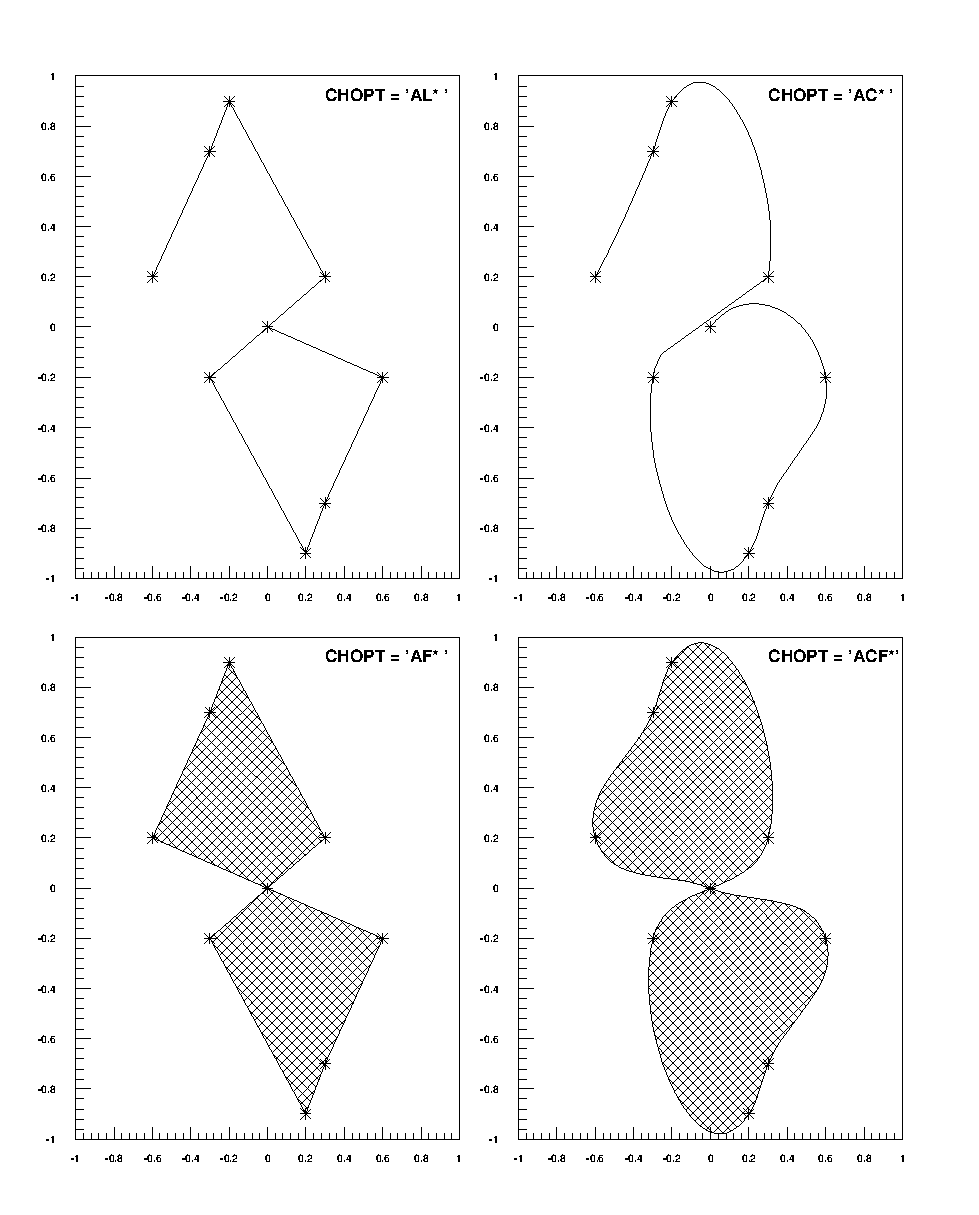
\epsfig{file=graph.eps}}
\end{center}
\caption{Example of \protect\Rind{IGRAPH} using {\tt L,C,F} and {\tt*} options.}
\label{GRAPH}
\end{figure}
\clearpage 

\Filename{H2Drawingahistogram}
\section{Drawing a histogram}
\index{histogram drawing}
\Shubr{IGHIST}{(N,X,Y,CHOPT)}
\Action
This routine draws a one-dimensional histogram with several possible 
presentations chosen by the user (histograms, bars, columns, smoothed graphs,
etc.).
\Pdesc
\begin{DLtt}{1234567}
\item[N] Number of bins in {\tt X} and/or {\tt Y}.
\item[X] Is either an array of dimension {\tt N} containing x
         coordinates or a two-dimensional array with {\tt (XMIN,XMAX)}
         (\WC~space).
\item[Y] Is either an array of dimension {\tt N} containing y
         coordinates or a two-dimensional array with {\tt (YMIN,YMAX)}
         (\WC~space).
\item[CHOPT] {\tt CHARACTER} variable specifying the options
             selected (Multiple simultaneous options are possible).
             Note that the number of components needed in the array {\tt X}
             and/or {\tt Y} may depend on the value of {\tt CHOPT}.
\begin{DLtt}{12345}
   \item['R'] The histogram is Rotated, i.e. the values in {\tt X} are used
              for the ordinate and the values in {\tt Y} for the abscissa
              (default is the contrary). If option {\tt 'R'} is selected (and
              option {\tt 'N'} is not selected), the user must give:
   \begin{UL}
      \item 2 values for {\tt Y} ({\tt Y(1)=YMIN} and {\tt Y(2)=YMAX})
      \item {\tt N} values for {\tt X}, one for each bin.
   \end{UL}
   Otherwise the user must give:
   \begin{UL}
      \item {\tt N} values for {\tt Y}, one for each bin.
      \item 2 values for {\tt X} ({\tt X(1)=XMIN} and {\tt X(2)=XMAX})
   \end{UL}
   For option {\tt 'N'} see below.
   \item['N'] Non equidistant bins (default is equidistant). The arrays {\tt X}
              and {\tt Y} must be dimensioned as follows:
              \\ If option {\tt R} is not selected (default) then the user
               must give:
   \begin{UL}
      \item ({\tt N+1}) values for {\tt X} (the limits of the bins).
      \item {\tt N} values for {\tt Y}, one for each bin.
   \end{UL}
   Otherwise the user must give:
   \begin{UL}
      \item ({\tt N+1}) values for {\tt Y} (the limits of the bins).
      \item {\tt N} values for {\tt X}, one for each bin.
   \end{UL}
   \item['H'] An histogram is drawn as a contour (default).
   \item['F'] The area delimited by the histogram is filled according to the
              fill area interior style and the fill area style index or colour
              index. The contour is not drawn unless the {\tt 'H'} option is
              also selected.
   \item['C'] A smooth curve is drawn across the points at the center of each
              bin of the histogram.
   \item['L'] A straight line is drawn across the points at the center of
              each bin of the histogram.
   \item['*'] A star is plotted at the center of each bin of the histogram.
   \item['P'] The current polymarker is plotted at the center of each bin
              of the histogram.
   \item['B'] A bar chart with equidistant bins is drawn as fill areas
              (contours are drawn). The bar origin and the bar
              width can be controlled by routine \Rind{IGSET} and the
              \Sind{BARO} and \Sind{BARW} options.
   \item['A'] The x and y axes are drawn.
   \item['GX'] Logarithmic scale on the X axis.
   \item['GY'] Logarithmic scale on the Y axis.
\end{DLtt}
\end{DLtt}

\begin{minipage}{\textwidth}
\begin{XMPt}{Example of {\tt HISTOGRAM} drawing (see result on figure 
\ref{HIST})}
      program hist 
      dimension x(2),y(10)
      parameter (xsize=16.,ysize=20.)
      data y/10.,30.,50.,400.,700.,900.,110.,90.,100.,40./
      data x/1.,1000./
*
      call start('hist',xsize,ysize)
*
*              Viewports definition
*
      xnorm  = min(1.,xsize/ysize)
      xnorm2 = xnorm/2.
      ynorm  = min(1.,ysize/xsize)
      ynorm2 = ynorm/2.
      rmarg  = 0.05
      rmarg2 = rmarg/2.
      call isvp(10,rmarg,xnorm2-rmarg2,ynorm2+rmarg2,ynorm-rmarg)
      call isvp(20,xnorm2+rmarg2,xnorm-rmarg,ynorm2+rmarg2,ynorm-rmarg)
      call isvp(30,rmarg,xnorm2-rmarg2,rmarg,ynorm2-rmarg2)
      call isvp(40,xnorm2+rmarg2,xnorm-rmarg,rmarg,ynorm2-rmarg2)
*
*              Some attributes setting
*
      call isclip(0)
      call igset('FASI',244.)
      call igset('FAIS',3.)
      call igset('CHHE',50.)
*
*              HISTOGRAM drawing
*
      call iswn(10,1.,1000.,1.,1000.)
      call iselnt(10)
      call ighist(10,x,y,'AHC*')
*
      call iswn(20,1.,1000.,1.,1000.)
      call iselnt(20)
      call ighist(10,x,y,'AB')
*
      call iswn(30,1.,1000.,log10(1.),log10(1000.))
      call iselnt(30)
      call ighist(10,x,y,'AHFGY')
*
      call iswn(40,log10(1.),log10(1000.),1.,1000.)
      call iselnt(40)
      call ighist(10,x,y,'AHFGX')
*
      call finish
      end
\end{XMPt}
\end{minipage}

\begin{figure}[p]
\begin{center}
\mbox{}\\[-15mm]
\mbox{\epsfig{file=hist.eps}}
\end{center}
\caption{Examples of \protect\Rind{IGHIST} usage.}
\label{HIST}
\end{figure}

\clearpage
 
\Filename{H2Bidimensionalmatrixdrawing}
\section{Bidimensional matrix drawing}
\index{2D matrix!drawing}
\Shubr{IGTABL}{(NX,NY,V,NPAR,PAR,CHOPT)}
\Action
This routine draws a 2D matrix (i.e. table) according to the values of
{\tt CHOPT} and {\tt PAR}. The {\tt PAR} input parameter could be specified 
to change the aspect of the plot (see the description below). The position of
the plot on the screen is given by the viewport of the current \NT~currently
selected (the window is not used and could be anything).
\Pdesc
\begin{DLtt}{12345678}
\item[NX]        Number of cells in X.
\item[NY]        Number of cells in Y.
\item[V(NX,NY)]  Content of the cells.
\item[NPAR]      Number of parameters in \Lit{PAR}.
\item[PAR(NPAR)] Array of real parameter. If \Lit{PAR(i)=0.} or \Lit{NPAR<i} a
                 default value is taken.
\item[CHOPT] {\tt CHARACTER} variable specifying the options selected. The
possible value of {\tt CHOPT} and the associate values of {\tt PAR} are
describe below. The default value of {\tt CHOPT} is \Lit{'P'}.
\end{DLtt}

\begin{XMPt}{Example of {\tt MATRIX} drawing (see result on figure 
\ref{SCATTER} to \ref{SURF4})}
      program matrix 
      call start_matrix('lego','LA')
      call start_matrix('lego1','L1A')
      call start_matrix('lego2','L2')
      call start_matrix('surf','SA')
      call start_matrix('surf1','S1A')
      call start_matrix('surf2','S2A')
      call start_matrix('surf3','S3A')
      call start_matrix('surf4','S4A')
      call start_matrix('surfpol','SPOL')
      call start_matrix('surfcyl','SCYL')
      call start_matrix('surfsph','SSPH')
      call start_matrix('surfpsd','SPSD')
      end

      subroutine start_matrix(name,chopt)
      character*(*) name,chopt
      parameter (nx=30,ny=30)
      dimension v(nx,ny)
      dimension par(29)
*
*              Parameters initialisation
*
      call vzero(par,29)
      par(1)=30.
      par(2)=23.
      par(3)=-10.
      par(4)=10.
      par(5)=-10
      par(6)=10.
      par(9)=1030.
      par(10)=1030.
      par(11)=510.
      par(12)=510.
      par(13)=510.
      par(14)=1.
      par(15)=1.
      par(16)=1.
      par(20)=0.05
      par(21)=-61.
      par(22)=.1
      par(23)=.1
      par(24)=.15
      par(25)=2.
      par(26)=5.
      par(27)=7.
      par(28)=6.
      par(29)=3.
*
*              Matrix filling
*
      x=-10.
      y=-10.
      s=20./float(nx)
      do i=1,nx
         do j=1,ny
            if(x.ne.0..and.y.ne.0)then
               v(i,j)=100.*sin(x)/x*sin(y)/y
            else
               v(i,j)=100.
            endif
            x=x+s
         enddo
         y=y+s
         x=-10.
      enddo
*
*              Matrix drawing
*
      call start(NAME,9.,9.)
      call isfais(0)
      call igset('BORD',1.)
      call igset('TXAL',32.)
      call igset('CHHE',0.25)
      call igtabl(nx,ny,v,29,par,chopt)
      call igterm
      call finish
      end
\end{XMPt}

\begin{figure}[p]
\begin{center}
\begin{tabular}{||c|p{12cm}|>{\tt}r||}
\hline
\multicolumn{3}{||l||}{\bf {\tt CHOPT = 'P'} Polymarker (scatter plot)}          \\
\hline
\multicolumn{1}{||c|}{\bf {\tt PAR} index}        &
\multicolumn{1}{c|}{\bf {\tt PAR} values}         &
\multicolumn{1}{c||}{\bf default}                \\
\hline
 1  & Marker type see \Rind{ISMK}.                                  &   1.    \\
 2  & Maximum number of random points per cell                      &   50.   \\
 3  & {\tt XMIN} Lowest X-axis label                                &   IXMIN \\
 4  & {\tt XMAX} Highest Y-axis label                               &   IXMAX \\
 5  & {\tt YMIN} Lowest Y-axis label                                &   IYMIN \\
 6  & {\tt YMAX} Highest Y-axis label                               &   IYMAX \\
 7  & {\tt ZMIN} Lowest Z value                                     &   ZMIN  \\
 8  & {\tt ZMAX} Highest Z value                                    &   ZMAX  \\
 9  & {\tt 1000*IXMIN + IXMAX} (Useful for ZOOM)                    &   1-NX  \\
 10 & {\tt 1000*IYMIN + IYMAX} (Useful for ZOOM)                    &   1-NY  \\
\hline
\end{tabular}
\end{center}

\bigskip

\begin{center} \mbox{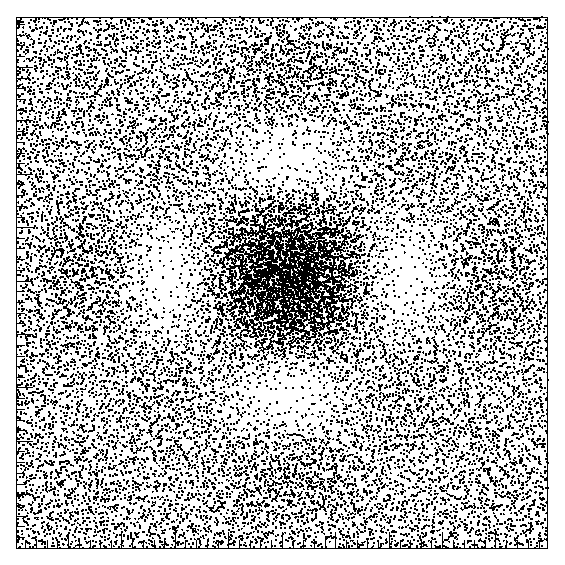
\epsfig{file=scatter.eps}} \end{center}
\caption{Example of the \protect\Rind{IGTABL} Polymarker option}
\label{SCATTER}
\end{figure}
 
\begin{figure}[p]
\begin{center}
\begin{tabular}{||c|p{12.cm}|>{\tt}r||}
\hline
\multicolumn{3}{||l||}{\bf {\tt CHOPT = 'B'} Boxes}               \\
\hline
\multicolumn{1}{||c|}{\bf {\tt PAR} index}              &
\multicolumn{1}{c|}{\bf {\tt PAR} values}               &
\multicolumn{1}{c||}{\bf default}                                 \\
\hline
 1  & Not used                                                      &         \\
 2  & Not used                                                      &         \\
 3  & {\tt XMIN} Lowest X-axis label                                &   IXMIN \\
 4  & {\tt XMAX} Highest Y-axis label                               &   IXMAX \\
 5  & {\tt YMIN} Lowest Y-axis label                                &   IYMIN \\
 6  & {\tt YMAX} Highest Y-axis label                               &   IYMAX \\
 7  & {\tt ZMIN} Lowest Z value                                     &   ZMIN  \\
 8  & {\tt ZMAX} Highest Z value                                    &   ZMAX  \\
 9  & {\tt 1000*IXMIN + IXMAX} (Useful for ZOOM)                    &   1-NX  \\
 10 & {\tt 1000*IYMIN + IYMAX} (Useful for ZOOM)                    &   1-NY  \\
\hline
\end{tabular}
\end{center}

\bigskip

\begin{center} \mbox{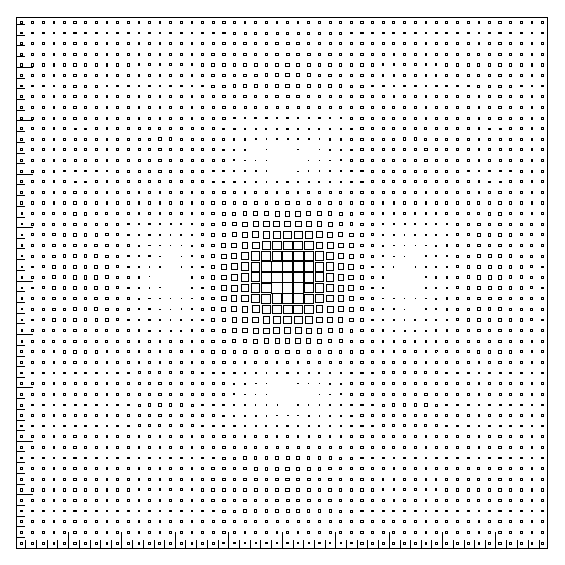
\epsfig{file=boxes.eps}} \end{center}
\caption{Example of the \protect\Rind{IGTABL} Boxes option}
\label{BOXES}
\end{figure}

\begin{figure}[p]
\begin{center}
\begin{tabular}{||c|p{12.cm}|>{\tt}r||}
\hline
\multicolumn{3}{||l||}{\bf {\tt CHOPT = 'R'} aRrows}       \\
\hline
\multicolumn{1}{||c|}{\bf {\tt PAR} index}       &
\multicolumn{1}{c|}{\bf {\tt PAR} values}        &
\multicolumn{1}{c||}{\bf default}                          \\
\hline
1  & Not used                                                       &         \\
2  & Not used                                                       &         \\
3  & XMIN Lowest X-axis label                                       &   IXMIN \\
4  & XMAX Highest Y-axis label                                      &   IXMAX \\
5  & YMIN Lowest Y-axis label                                       &   IYMIN \\
6  & YMAX Highest Y-axis label                                      &   IYMAX \\
7  & ZMIN Lowest Z value                                            &   ZMIN  \\
8  & ZMAX Highest Z value                                           &   ZMAX  \\
9  & 1000*IXMIN + IXMAX (Useful for ZOOM)                           &   1-NX  \\
10 & 1000*IYMIN + IYMAX (Useful for ZOOM)                           &   1-NY  \\
\hline
\end{tabular}
\end{center}

\bigskip

\begin{center} \mbox{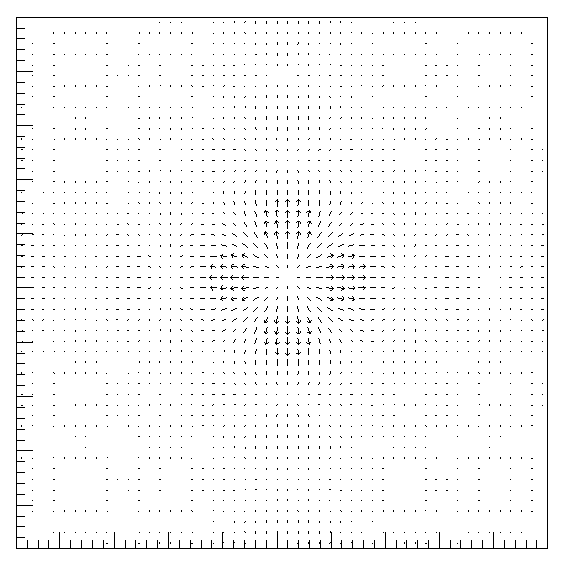
\epsfig{file=arrows.eps}} \end{center}
\caption{Example of the \protect\Rind{IGTABL} aRrows option}
\label{ARROWS}
\end{figure}

\begin{figure}[p]
\begin{center}
\begin{tabular}{||c|p{12.cm}|>{\tt}r||}
\hline
\multicolumn{3}{||l||}{\bf {\tt CHOPT = 'C'} Contour plot}     \\
\hline
\multicolumn{1}{||c|}{\bf {\tt PAR} index}           &
\multicolumn{1}{c|}{\bf {\tt PAR} values}            &
\multicolumn{1}{c||}{\bf default}                              \\
\hline
1    & Nlevel (min=2 max=50)                                        &   20.   \\
2    & 0 use colour to distinguish contours. Line type used is 1.   &    0.   \\
     & 1.XXX use line style to distinguish contours.
       Colour index used is \Lit{XXX}.                              &         \\
     & 2.XXX line style and colour are the same for all contours.   &         \\
     & Colour index used is \Lit{XXX}.                              &         \\
3    & XMIN Lowest X-axis label                                     &   IXMIN \\
4    & XMAX Highest Y-axis label                                    &   IXMAX \\
5    & YMIN Lowest Y-axis label                                     &   IYMIN \\
6    & YMAX Highest Y-axis label                                    &   IYMAX \\
7    & ZMIN Lowest Z value                                          &   ZMIN  \\
8    & ZMAX Highest Z value                                         &   ZMAX  \\
9    & 1000*IXMIN + IXMAX (Useful for ZOOM)                         &   1-NX  \\
10   & 1000*IYMIN + IYMAX (Useful for ZOOM)                         &   1-NY  \\
\hline
\end{tabular}
\end{center}

\bigskip

\begin{center} \mbox{\epsfig{file=contour.eps}} \end{center}
\caption{Example of the \protect\Rind{IGTABL} Contour option}
\label{CONTOUR}
\end{figure}

\begin{figure}[p]
\begin{center}
\begin{tabular}{||c|p{12.cm}|>{\tt}r||}
\hline
\multicolumn{3}{||l||}{\bf {\tt CHOPT = 'COL'} COLour plot}    \\
\hline
\multicolumn{1}{||c|}{\bf {\tt PAR} index}           &
\multicolumn{1}{c|}{\bf {\tt PAR} values}            &
\multicolumn{1}{c||}{\bf default}                              \\
\hline
1  & 0 use the standard 8 colours                                   &   0.    \\
2  & ...                                                            &         \\
3  & XMIN Lowest X-axis label                                       &   IXMIN \\
4  & XMAX Highest Y-axis label                                      &   IXMAX \\
5  & YMIN Lowest Y-axis label                                       &   IYMIN \\
6  & YMAX Highest Y-axis label                                      &   IYMAX \\
7  & ZMIN Lowest Z value                                            &   ZMIN  \\
8  & ZMAX Highest Z value                                           &   ZMAX  \\
9  & 1000*IXMIN + IXMAX (Useful for ZOOM)                           &   1-NX  \\
10 & 1000*IYMIN + IYMAX (Useful for ZOOM)                           &   1-NY  \\
\hline
\end{tabular}
\end{center}
\index{colour!matrix drawing}

\bigskip

\begin{center} \mbox{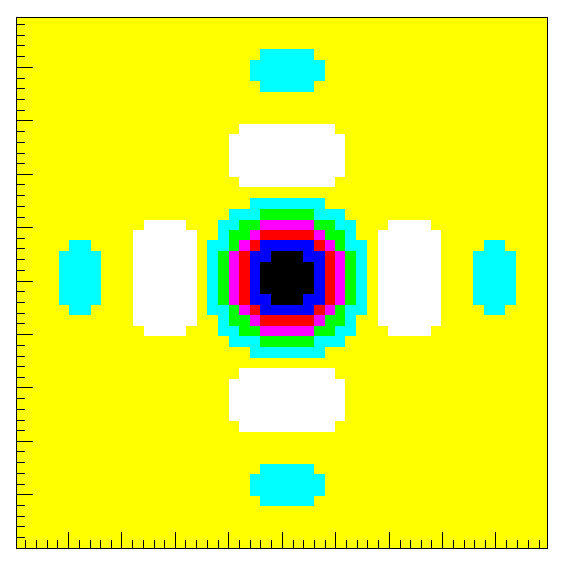
\epsfig{file=colour.eps}} \end{center}
\caption{Example of the \protect\Rind{IGTABL} COLour option}
\label{COLOUR}
\end{figure}

\begin{figure}[p]
\begin{center}
\begin{tabular}{||c|p{12.cm}|>{\tt}r||}
\hline
\multicolumn{3}{||l||}{\bf {\tt CHOPT = 'T'} Text}             \\
\hline
\multicolumn{1}{||c|}{\bf {\tt PAR} index}           &
\multicolumn{1}{c|}{\bf {\tt PAR} values}            &
\multicolumn{1}{c||}{\bf default}                              \\
\hline
1  & Text font                                                      &   1.    \\
2  & Text Precision                                                 &   0.    \\
3  & XMIN Lowest X-axis label                                       &   IXMIN \\
4  & XMAX Highest Y-axis label                                      &   IXMAX \\
5  & YMIN Lowest Y-axis label                                       &   IYMIN \\
6  & YMAX Highest Y-axis label                                      &   IYMAX \\
7  & ZMIN Lowest Z value                                            &   ZMIN  \\
8  & ZMAX Highest Z value                                           &   ZMAX  \\
9  & 1000*IXMIN + IXMAX (Useful for ZOOM)                           &   1-NX  \\
10 & 1000*IYMIN + IYMAX (Useful for ZOOM)                           &   1-NY  \\
\hline
\end{tabular}
\end{center}

\bigskip

\begin{center} \mbox{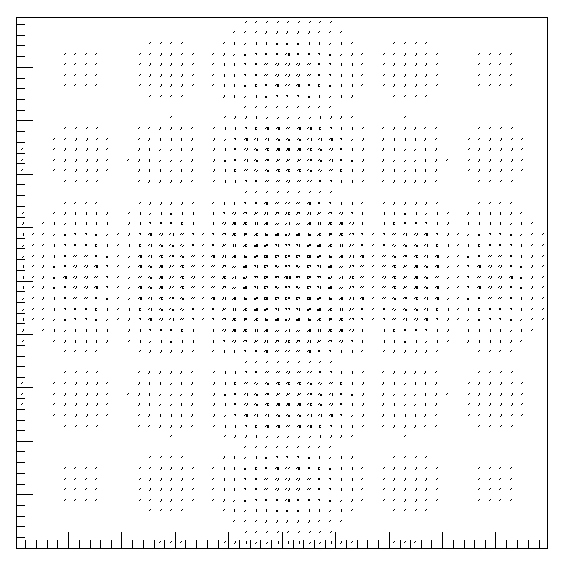
\epsfig{file=tabt.eps}} \end{center}
\caption{Example of the \protect\Rind{IGTABL} Text option}
\label{TABT}
\end{figure}

\begin{figure}[p]
\begin{center}
\begin{tabular}{||c|p{12.cm}|>{\tt}r||}
\hline
\multicolumn{3}{||l||}{\bf {\tt CHOPT = 'K'} character}     \\
\hline
\multicolumn{1}{||c|}{\bf {\tt PAR} index}        &
\multicolumn{1}{c|}{\bf {\tt PAR} values}         &
\multicolumn{1}{c||}{\bf default}                           \\
\hline
1  & Text font                                                      &   1.    \\
2  & Text Precision                                                 &   0.    \\
3  & XMIN Lowest X-axis label                                       &   IXMIN \\
4  & XMAX Highest Y-axis label                                      &   IXMAX \\
5  & YMIN Lowest Y-axis label                                       &   IYMIN \\
6  & YMAX Highest Y-axis label                                      &   IYMAX \\
7  & ZMIN Lowest Z value                                            &   ZMIN  \\
8  & ZMAX Highest Z value                                           &   ZMAX  \\
9  & 1000*IXMIN + IXMAX (Useful for ZOOM)                           &   1-NX  \\
10 & 1000*IYMIN + IYMAX (Useful for ZOOM)                           &   1-NY  \\
\hline
\end{tabular}
\end{center}

\bigskip

\begin{center} \mbox{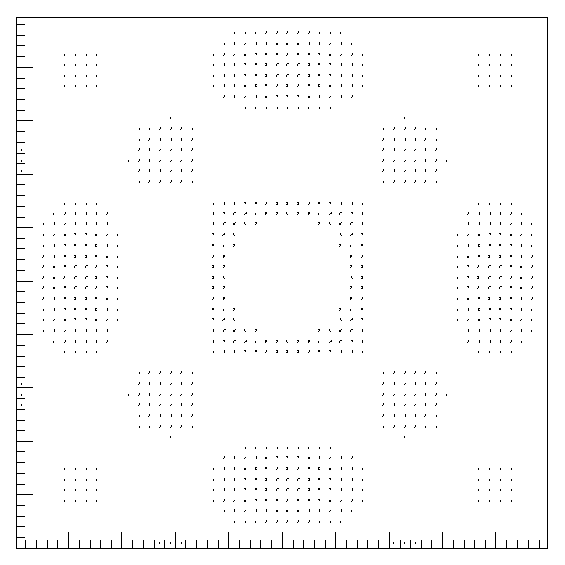
\epsfig{file=tabk.eps}} \end{center}
\caption{Example of the \protect\Rind{IGTABL} character \protect\Lit{K} option}
\label{TABK}
\end{figure}

\begin{table}[p]
\begin{center}
\begin{tabular}{||c|p{12.cm}|>{\tt}r||}
\hline
\multicolumn{3}{||l||}
{\bf {\tt CHOPT = 'L'} Lego (mode 0)}                                         \\
\multicolumn{3}{||l||}
{\bf {\tt CHOPT = 'LB'} Lego with BARO and BARW}                              \\
\multicolumn{3}{||l||}
{\bf {\tt CHOPT = 'L1'} Lego with colours (mode 1)}                           \\
\multicolumn{3}{||l||}
{\bf {\tt CHOPT = 'L2'} Lego with colours (mode 2)}                           \\
\hline
\multicolumn{3}{||l||}
{\bf {\tt CHOPT = 'S'} Surface (mode 0)}                                      \\
\multicolumn{3}{||l||}
{\bf {\tt CHOPT = 'S1'} Surface with colours (mode 1)}                        \\
\multicolumn{3}{||l||}
{\bf {\tt CHOPT = 'S2'} Surface with colours (mode 2)}                        \\
\multicolumn{3}{||l||}
{\bf {\tt CHOPT = 'S3'} Surface with contour plot on top (mode 3)}            \\
\multicolumn{3}{||l||}
{\bf {\tt CHOPT = 'S4'} Surface with Gouraud shading (mode 4)}                \\
\hline
\multicolumn{3}{||l||}
{\bf {\tt CHOPT = 'CYL'} Cylindrical for lego and surface}                    \\
\multicolumn{3}{||l||}
{\bf {\tt CHOPT = 'SPH'} Spherical for lego and surface}                      \\
\multicolumn{3}{||l||}
{\bf {\tt CHOPT = 'PSD'} Pseudo rapidity for lego and surface}                \\
\hline
\multicolumn{1}{||c|}{\bf {\tt PAR} index}       &
\multicolumn{1}{c|}{\bf {\tt PAR} values}        &
\multicolumn{1}{c||}{\bf default}                          \\
\hline
1  & {\tt THETA}                                                    &   30.   \\
2  & {\tt PHI}                                                      &   30.   \\
3  & {\tt XMIN} Lowest X-axis label                                 &   IXMIN \\
4  & {\tt XMAX} Highest Y-axis label                                &   IXMAX \\
5  & {\tt YMIN} Lowest Y-axis label                                 &   IYMIN \\
6  & {\tt YMAX} Highest Y-axis label                                &   IYMAX \\
7  & {\tt ZMIN} Lowest Z value                                      &   ZMIN  \\
8  & {\tt ZMAX} Highest Z value                                     &   ZMAX  \\
9  & {\tt 1000*IXMIN + IXMAX} (Useful for ZOOM)                     &   1-NX  \\
10 & {\tt 1000*IYMIN + IYMAX} (Useful for ZOOM)                     &   1-NY  \\
11 & {\tt NDVX}                                                     &  510.00 \\
12 & {\tt NDVY}                                                     &  510.00 \\
13 & {\tt NDVZ}                                                     &  510.00 \\
14 & {\tt XCOL}                                                     &    1.00 \\
15 & {\tt YCOL}                                                     &    1.00 \\
16 & {\tt ZCOL}                                                     &    1.00 \\
17 & {\tt XTIC}                                                     &    0.02 \\
18 & {\tt YTIC}                                                     &    0.02 \\
19 & {\tt ZTIC}                                                     &    0.02 \\
20 & {\tt VSIZ}                                                     &    0.02 \\
21 & {\tt VFON}                                                     &    2.00 \\
22 & {\tt XVAL}                                                     &    0.02 \\
23 & {\tt YVAL}                                                     &    0.02 \\
24 & {\tt ZVAL}                                                     &    0.04 \\
25 & Palette                                                        &    0.04 \\
\hline
\end{tabular}
\end{center}
\caption{Values of the \protect\Rind{IGTABL} Lego and Surface option}
\label{tab-IGTABLS}
\end{table}

\begin{figure}[p]
\begin{center}\mbox{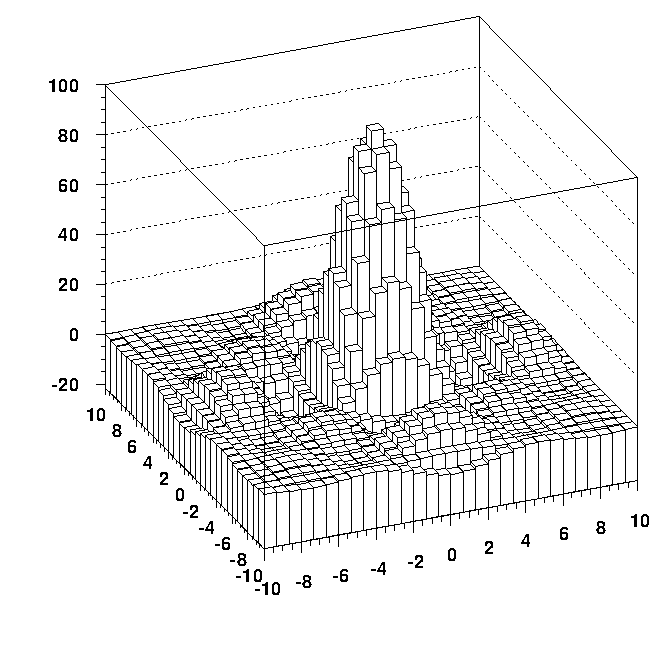
\epsfig{file=lego.eps}}\end{center}
\caption{Example of the \protect\Rind{IGTABL} Lego option}
\label{LEGO}
\begin{center}\mbox{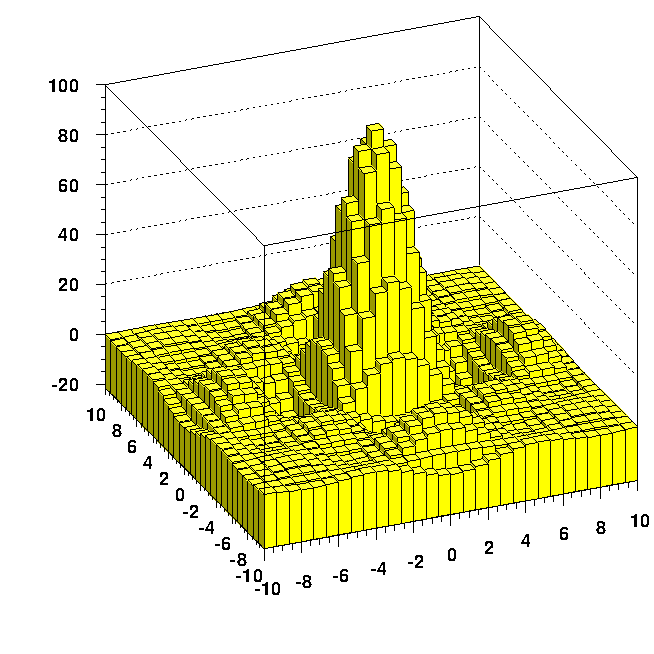
\epsfig{file=lego1.eps}}\end{center}
\caption{Example of the \protect\Rind{IGTABL} Lego \protect\Lit{L1} option}
\label{LEGO1}
\end{figure}

\begin{figure}[p]
\begin{center}\mbox{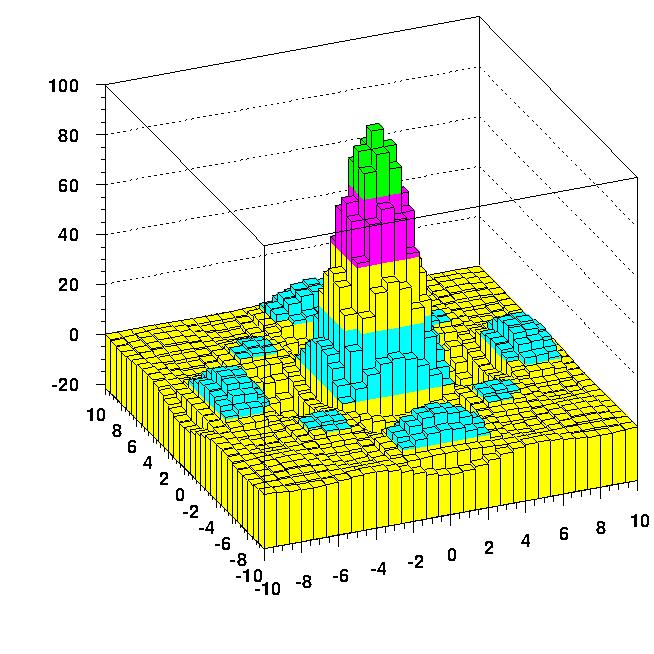
\epsfig{file=lego2.eps}}\end{center}
\caption{Example of the \protect\Rind{IGTABL} Lego \protect\Lit{L2} option}
\label{LEGO2}
\begin{center}\mbox{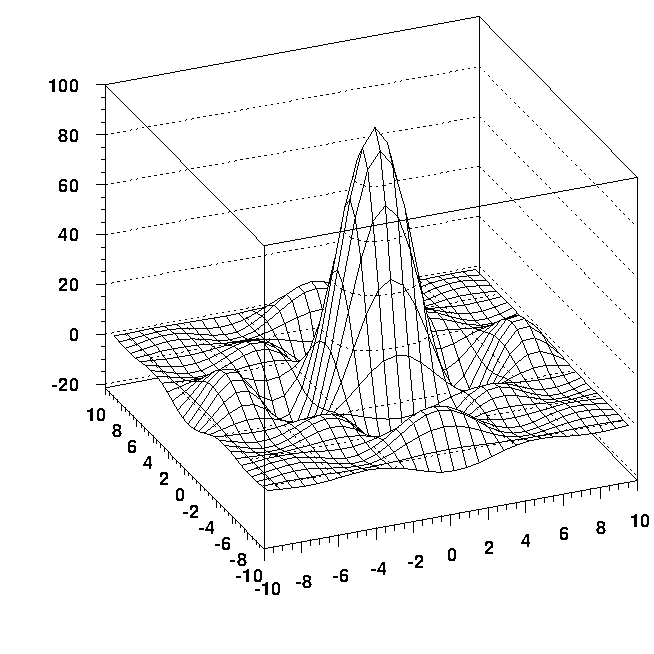
\epsfig{file=surf.eps}}\end{center}
\caption{Example of the \protect\Rind{IGTABL} Surface option}
\label{SURF}
\end{figure}

\begin{figure}[p]
\begin{center}\mbox{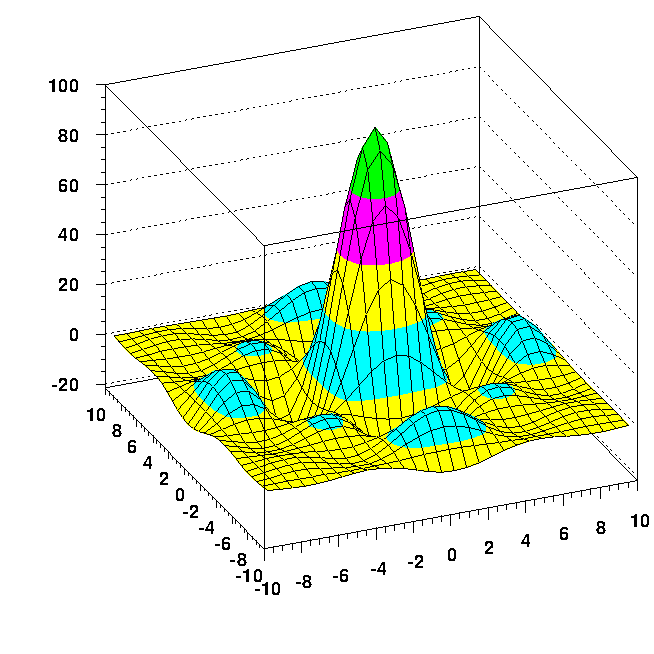
\epsfig{file=surf1.eps}}\end{center}
\caption{Example of the \protect\Rind{IGTABL} Surface \protect\Lit{S1} option}
\label{SURF1}
\begin{center}\mbox{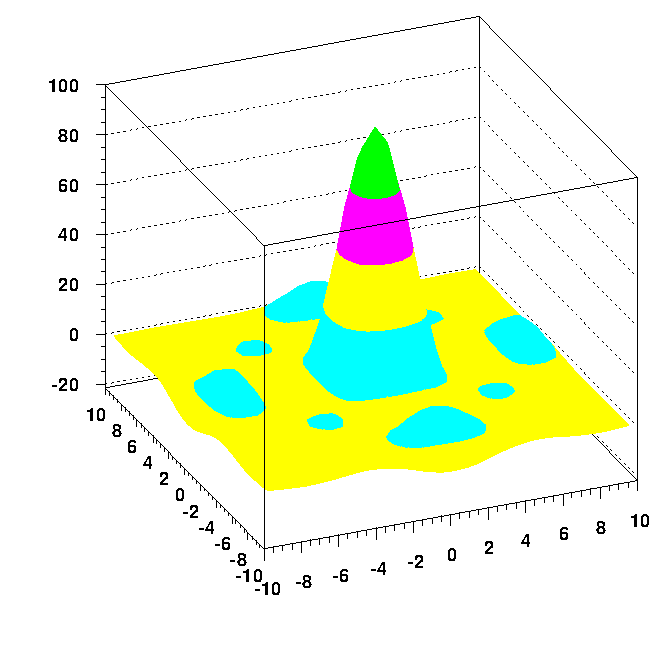
\epsfig{file=surf2.eps}}\end{center}
\caption{Example of the \protect\Rind{IGTABL} Surface \protect\Lit{S2} option}
\label{SURF2}
\end{figure}

\begin{figure}[p]
\begin{center}\mbox{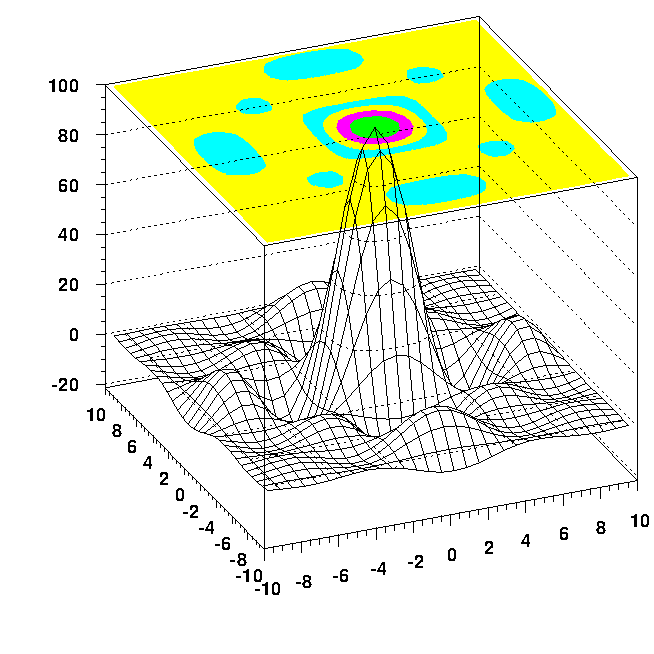
\epsfig{file=surf3.eps}}\end{center}
\caption{Example of the \protect\Rind{IGTABL} Surface \protect\Lit{S3} option}
\label{SURF3}
\begin{center}\mbox{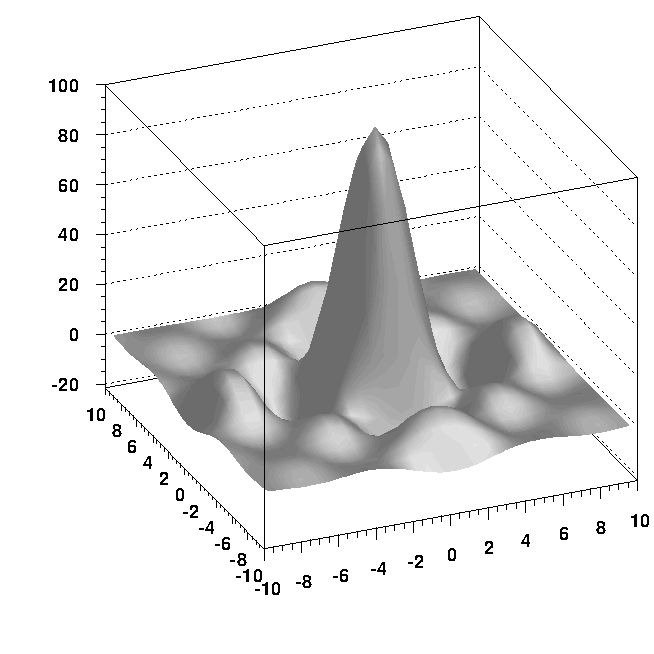
\epsfig{file=surf4.eps}}\end{center}
\caption{Example of the \protect\Rind{IGTABL} Surface \protect\Lit{S4} option}
\label{SURF4}
\end{figure}

\begin{figure}[p]
\begin{center}\mbox{\epsfig{file=surfpol.eps}}\end{center}
\caption{Example of the \protect\Rind{IGTABL} Surface \protect\Lit{SPOL} option}
\label{SPOL}
\begin{center}\mbox{\epsfig{file=surfcyl.eps}}\end{center}
\caption{Example of the \protect\Rind{IGTABL} Surface \protect\Lit{SCYL} option}
\label{SCYL}
\end{figure}

\begin{figure}[p]
\begin{center}\mbox{\epsfig{file=surfsph.eps}}\end{center}
\caption{Example of the \protect\Rind{IGTABL} Surface \protect\Lit{SSPH} option}
\label{SSPH}
\begin{center}\mbox{\epsfig{file=surfpsd.eps}}\end{center}
\caption{Example of the \protect\Rind{IGTABL} Surface \protect\Lit{SPSD} option}
\label{SPSD}
\end{figure}

Note that the options \Lit{POL}, \Lit{CYL}, \Lit{SPH}, and \Lit{PSD} can be
used together with any lego or surface options.
\clearpage

\begin{Tabhere}
\begin{tabularx}{\textwidth}{||c|X||}
\hline
 \Lit{CHOPT} &                Description                                           \\
\hline
  'H'  & Data are compacted as in \HPLOT.                                     \\
\hline
  'GX' & loG on X coordinates. A log \WC~must be defined before.              \\
\hline
  'GY' & loG on Y coordinates. A log \WC~must be defined before.              \\
\hline
  'GZ' & loG on Z coordinates.                                                \\
\hline
  'A'  & 2nd vertical axis (legos and Surfaces only)                          \\
       & axis (for the 2D representations).                                   \\
\hline
  '+'  & For stacked histograms (legos).                                      \\
\hline
  'Z'  & Allows to display the Z scale.                                       \\
\hline
\end{tabularx}
\caption{Other options for \protect\Rind{IGTABL}}
\label{tab-IGTABL}
\end{Tabhere}

\begin{XMPt}{Example of stacked lego plots drawing (see result on figure 
\ref{STACK})}
      program stack 
      parameter (nx=10,ny=10)
      parameter (npar=25)
      dimension v1(nx,ny),v2(nx,ny),v3(nx,ny)
      dimension par(npar)
      call vzero(par,npar)
      par(1)  = 30.
      par(2)  = 23.
      par(3)  = -10.
      par(4)  = 10.
      par(5)  = -10
      par(6)  = 10.
      par(9)  = 1000. + nx
      par(10) = 1000. + ny
      par(11) = 510.
      par(12) = 510.
      par(13) = 510.
      par(14) = 1.
      par(15) = 1.
      par(16) = 1.
      par(20) = 0.05
      par(21) = -61.
      par(22) = .1
      par(23) = .15
      par(24) = .1
*
*              Matrices filling
*
      do i=1,nx
         do j=1,ny
            v1(i,j)=float(i)
            v2(i,j)=float(i+j)
            v3(i,j)=float(j)
         enddo
      enddo
*
*              Stack drawing
*
      call start('stack',9.,9.)
      call igset('BARW',0.5)
      par(25) = 2.
      call igtabl(nx,ny,v1,npar,par,'+')
      par(25) = 5.
      call igtabl(nx,ny,v2,npar,par,'+')
      par(25) = 3.
      call igtabl(nx,ny,v3,npar,par,'LB1A')
      call igterm
      call finish
*
      end
\end{XMPt}

\begin{Fighere}
\begin{center}\mbox{\epsfig{file=stack.eps}}\end{center}
\caption{Example of stacked lego plots}
\label{STACK}
\end{Fighere}
\clearpage

\Filename{H2Drawingapiechart}
\section{Drawing a pie chart}
\index{pie chart drawing}
\Shubr{IGPIE}{(X0,Y0,RADIUS,N,VALUES,CHOPT,IAO,IAS,IAC)}
\Action
This routine draws a graph in form of a pie chart.
\Pdesc
\begin{DLtt}{1234567}
\item[X0]     X coordinate of the center of the pie chart.
\item[Y0]     Y coordinate of the center of the pie chart.
\item[RADIUS] Radius of the pie chart.
\item[N]      Number of entries in the array {\tt VALUES}
\item[VALUES] Array of dimension {\tt N} containing the values determining
              the size of the slices in the pie.
\item[CHOPT]  Character variable specifying the combination of options
              desired:
\begin{DLtt}{12345}
\item['C'] Colours array is present.
\item['L'] Alphanumeric labels are required (see section \ref{IGLBL}).
\item['O'] Offset array is present.
\item['N'] The label of each slice will be the corresponding numeric value in
           array {\tt VALUES}.
\item['P'] The label of each slice will be in expressed in percentage.
\item['S'] Style array is present.
\item['H'] Force the labels size to be the current character height. Without
           this option the labels size is computed automatically.
\item['R'] Draw the labels aligned on the radius of each slice.
\end{DLtt}
\item[IAO] Array of dimension {\tt N} containing offsets of the corresponding
           slice in percentage of the radius.
\item[IAS] Array of dimension {\tt N} containing the interior style index for
           every slice.
\item[IAC] Array of dimension {\tt N} containing the colour index for every
           slice.
\end{DLtt}
\newpage

\begin{XMPt}{Example of {\tt PIE CHART} drawing (see result on figure \ref{PIE}}
      program  pie 
      dimension v(8),iao(8),ias(8)
      data v /1.,1.8,2.9,1.,1.8,2.9,1.,1.8/
      data iao /0,0,0,20,0,0,20,0/
      data ias /205,295,245,244,254,245,244,245/
      call start('pie',12.,9.)
      call isclip(0)
      call igbox(0.,12.,0.,9.)
      call igset('BORD',1.)
      call igpie(3.,6.,2.,8,v,'OSN',iao,ias,0)
      call igpie(9.,6.,2.,8,v,'OSP',iao,ias,0)
      call igset('TXAL',23.)
      call igset('CHHE',0.3)
      call itx(3.,3.,'CHOPT = ''OSN''')
      call itx(9.,3.,'CHOPT = ''OSP''')
      call itx(6.,2.,'IAO = 0,0,0,20,0,0,20,0')
      call itx(6.,1.,'IAS = 205,295,245,244,254,245,244,245')
      call finish
      end
\end{XMPt}

\begin{Fighere}
\begin{center}
\mbox{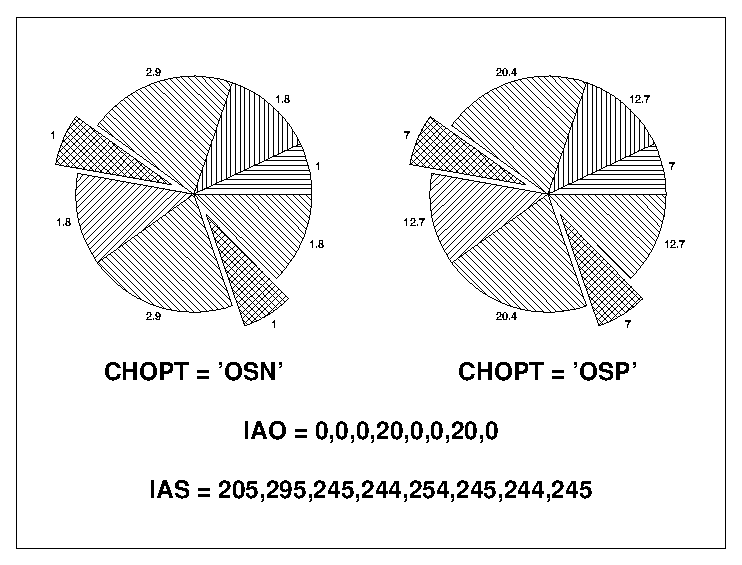
\epsfig{file=pie.eps,height=9cm}}
\end{center}
\caption{Examples of \protect\Rind{IGPIE}}
\label{PIE}
\end{Fighere}
\clearpage
 
\Filename{H2Drawingaxes}
\section{Drawing axes}
\index{axis drawing}
\Shubr{IGAXIS}{(X0,X1,Y0,Y1,WMIN,WMAX,NDIV,CHOPT)}
\Action
This routines allows the user to draw axes on a picture.
\Pdesc
\begin{DLtt}{1234567}
\item[X0]   X coordinate of the origin of the axis in \WC~space.
\item[X1]   X coordinate of the end of the axis in \WC~space.
\item[Y0]   Y coordinate of the origin of the axis in \WC~space.
\item[Y1]   Y coordinate of the end of the axis in \WC~space.
\item[WMIN] Lowest value for the tick mark labels written on the axis.
\item[WMAX] Highest value for the tick mark labels written on the axis.
\item[NDIV] Number of divisions. calculated according to the following
            convention:
\begin{DLtt}{123}
\item[NDIV = N1 + 100*N2 + 10000*N3] where,
\item[N1] Number of primary divisions.
\item[N2] Number of second order divisions.
\item[N3] Number of third order divisions.
\end{DLtt}
Examples:
\begin{DLtt}{1234567}
\item[NDIV=0] No tick marks.
\item[NDIV=2] produces 2 divisions with one tick mark in the middle of the axis.
\end{DLtt}
Note that, in case numeric labels are requested, {\tt N1} indicates the maximum
number of primary divisions. An appropriate algorithm calculates a number of
primary divisions less or equal to N1, in order to obtain ``reasonable'' labels.
Option {\tt'N'} in {\tt CHOPT} forces {\tt N1} to be used as the {\bf exact}
number of primary divisions.
\item[CHOPT] Character variable specifying the combinations of options desired.
\par {\bf General options}
\begin{DLtt}{12345}
\item['G'] LoGarithmic scale, default is linear.
\item['B'] Blank axis, i.e. the base line constituting the axis is not drawn.
           However tick marks and labels are drawn. Useful when superimposing
           two axes.
\item['A'] An arrow is drawn at the end of the axis (position {\tt WMAX}).
\item['N'] N1 will be used as exact number of divisions.
\end{DLtt}
 
{\bf Orientation of the tick marks on the axis }
\index{axis!tick marks!orientation}
 
Tick marks are normally drawn on the positive side of the axis. However, if the
axis is vertical, i.e. if {\tt X0=X1}, then they are drawn on the ``negative''
side. Their orientation can be selected by {\tt CHOPT}.
\begin{DLtt}{12345}
\item['+'] Tick marks are drawn on the positive side of the axis (default).
\item['-'] Tick marks are drawn on the negative side of the axis.
\end{DLtt}
Specifying {\tt'+-'} will draw tick marks on {\bf both} sides of the axis.
 
{\bf Orientation of tick marks and labels in the working space }
\index{axis!tick marks!orientation}
\index{axis!labels!orientation}
 
Tick marks are normally drawn orthogonal to the axis.
However, in case of an oblique axis, they can be drawn vertically.
\begin{DLtt}{12345}
\item['V'] Tick marks are drawn Vertically (default is perpendicular to axis).
\end{DLtt}
 
\newpage
{\bf Labeling an axis }
\index{axis!labeling}
 
An axis is normally labeled, unless specified otherwise:
\begin{DLtt}{12345}
\item['U'] Unlabeled axis (default is labeled).
\end{DLtt}
 
{\bf Position of labels on an axis }
\index{axis!labels!position}
 
Labels are normally drawn on the side opposite to the tick marks,
unless specified otherwise:
\begin{DLtt}{12345}
\item['='] Labels are drawn on the same side as the tick marks.
\end{DLtt}
 
{\bf Orientation of labels on an axis. }
\index{axis!labels!orientation}
 
Labels are normally drawn parallel to the axis.
 
However if the axis is vertical, i.e.
if {\tt X0=X1}, then the labels are drawn
orthogonally. If the axis is horizontal, i.e. if {\tt Y0=Y1}, then the
labels are Parallel to the axis:
\begin{DLtt}{12345}
\item['P'] Labels are drawn Parallel to the axis
\item['O'] Labels are drawn Orthogonal to the axis.
\end{DLtt}
 
{\bf Position of labels with respect to the tick marks. }
\index{axis!labels!position}
 
Labels are centered on tick marks. However,
if the axis is vertical ({\tt X0=X1}), then they are right adjusted.
\begin{DLtt}{12345}
\item['R'] Labels are Right adjusted on a tick mark.
\item['L'] Labels are Left adjusted on a tick mark.
\item['C'] Labels are centered on tick a mark. (default)
\end{DLtt}
 
{\bf Direction of labels }
\index{axis!labels!direction}
 
The default writing direction of labels is from {\bf left to right}.
\begin{DLtt}{12345}
\item['Y'] Writing direction is {\bf downwards}.
\end{DLtt}
 
{\bf Format of labels }
\index{axis!labels!format}
 
Training blanks in the label strings are stripped, and then the label is
correctly aligned. If the last character of the string is a dot {\tt'.'},
it is also stripped by default.
\begin{DLtt}{12345}
\item['.'] The dot at the end of a string is mandatory.
\end{DLtt}
 
{\bf Type of labels }
\index{axis!labels!type}
\index{axis!labels!alphanumeric}
 
Labels are by default numeric.
\begin{DLtt}{12345}
\item['T'] The labels are alphanumeric text strings. In this case 12 default
           values are provided, namely the 3-character abbreviations of the
           names of the months: {\tt'JAN'}, {\tt'FEB'}, {\tt'MAR'},\ldots.
           These values can be modified by calling the routine \Rind{IGLBL}
           (see section \ref{IGLBL}).
\end{DLtt}
 
{\bf Optional grid }
\index{grid|see{axis grid}}
 
An optional grid (cross-wires) can be drawn as a prolongation of the primary
tick marks.
\begin{DLtt}{12345}
\item['W'] Draw cross-wires at the position of the primary tick marks.
           The length of the grid can be defined, in \WC, with the
           \Rind{IGSET} parameter \Sind{AWLN}. The current line type
           is used to draw the grid.
\end{DLtt}
 
{\bf Intrinsic parameters }
\index{axis!intrinsic parameters}
 
The default values for \HIGZ~intrinsic parameter settings are shown below
expressed as a percentage of the length of the axis (\WC):
\begin{DL}{\bf Characters height for labels:M}
\item[Primary tick marks:] 3.0 \%
\item[Secondary tick marks:]1.5 \%
\item[Third order tick marks:].75 \%
\item[Length of the arrow:]3.0 \%
\item[Width of the arrow:].75 \%
\item[Characters height for labels:] 2.0 \%
\item[Characters spacing:] 40\% of the character height
\item[Labels offset:] 4.0 \%
\end{DL}
 
The size of the secondary tick marks is always 50\% of the primary ones. The
size of the third order tick marks is always 50\% of the secondary ones.
 
These values can be changed by calls to routine \Rind{IGSET}. The default value
is used {\bf unless } the corresponding option is selected by {\tt CHOPT}:
\begin{DLtt}{12345}
\item['D'] The distance between the labels and the axis (the offset) is given by
           the preceding call to \Rind{IGSET} with the parameter \Sind{LAOF}.
\item['H'] The size (height) of the labels is given by the preceding call to
           \Rind{IGSET} with the parameter \Sind{LASI}.
\item['S'] The size of the tick marks is given by the preceding call to
           \Rind{IGSET} with the parameter \Sind{TMSI}.
\end{DLtt}
\end{DLtt}
 
\subsection{Control of Alphanumeric labels}
\index{axis!labels!alphanumeric}
\Shubr{IGLBL}{(NLBL,CHLBL)}
\Action
This routine must be called to alter the values of the alphanumeric labels used
in \Rind{IGAXIS}.
\Pdesc
\begin{DLtt}{1234567}
\item[NLBL] Number of alphanumeric labels specified in array {\tt CHLBL}.
            The number of labels is limited to 50.
\item[CHLBL] {\tt CHARACTER} array containing the new values for the
             alphanumeric labels. The maximal length of each label is 32
             characters.
\end{DLtt}

\newpage

\begin{XMPt}{Example of {\tt AXIS} drawing (see result on figure \ref{AXIS})}
      program axis 
      call start('axis',12.,12.)
      call igbox(0.,12.,0.,12.)
      call igaxis (1.,11.,1.,1.,0.,100.,510,'A')
      call igaxis (1.,11.,3.,3.,1.,10000.,510,'G')
      call igaxis (1.,11.,5.,5.,0.,12.,11,'NATY')
      call igaxis (1.,11.,6.,6.,-100.,0.,510,'A')
      call igaxis (11.,1.,7.,7.,-100.,0.,810,'A+-')
      call igaxis (1.,11.,8.,11.,0.,1234567.,615,'A')
      call igaxis (6.,11.,8.5,8.5,-3.14,0.,50505,'AN')
      call finish
      end
\end{XMPt}
 
\begin{Fighere}
\begin{center}
\mbox{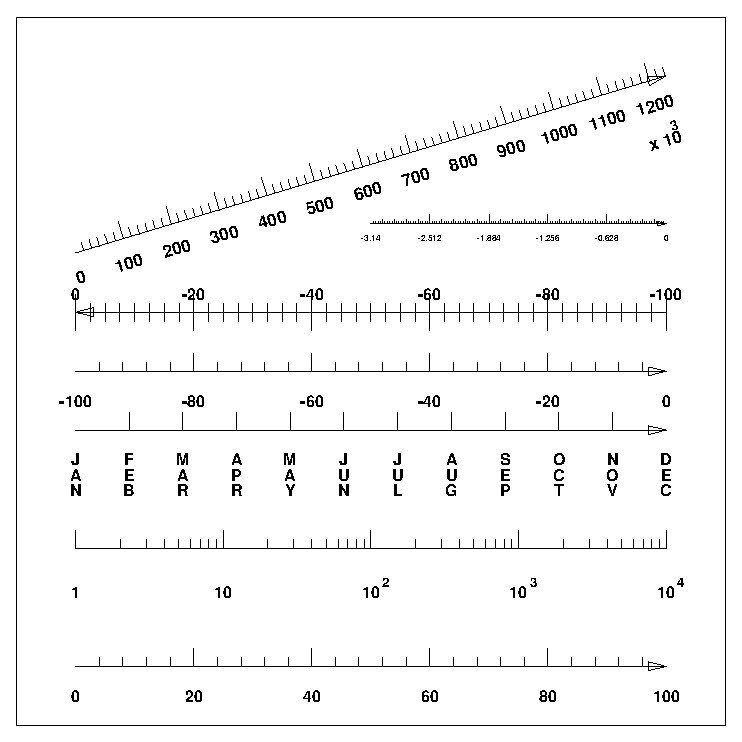
\epsfig{file=axis.eps,height=12cm}}
\end{center}
\caption{Examples of \protect\Rind{IGAXIS}}
\label{AXIS}
\end{Fighere}
 
\newpage

\Filename{H2Drawingsoftwarecharacters}
\section{Drawing software characters}
\index{text!software characters}
\Shubr{IGTEXT}{(X,Y,CHARS,SIZE,ANGLE,CHOPT)}
\Action
This routine draws a software character text, independently from \UGP{} used by
\HIGZ. \Rind{IGTEXT} can produce over 300 different graphic signs.
The way in which software characters are defined is via a string of valid
\FORTRAN{} characters, intermixed by other valid \FORTRAN{} characters, acting as
``escape'' characters \index{character!escape} (e.g. a change of
alphabet, upper or lower case). The string is interpreted by \Rind{IGTEXT} and
the resulting characters are defined according to the figure~\ref{SOFTTEXT},
which shows the list of available software characters. This routine allows the
user to mix different types of characters (roman, greek, special, upper and
lower case, sub and superscript). There are a total of 10 control characters.
\Pdesc
\begin{DLtt}{1234567}
\item[X] x coordinate in \WC space.
\item[Y] y coordinate in \WC space.
\item[CHARS] {\tt CHARACTER} variable containing the text
to be displayed.
\item[SIZE] Size of the text in \WC space.
\item[ANGLE] Inclination angle of the text inclination in degrees.
\item[CHOPT] {\tt CHARACTER} variable specifying the text alignment:
\begin{DLtt}{12345}
\item['L'] The text is Left adjusted starting at the point {\tt(X,Y)}.
\item['C'] The text is Centered around the the point {\tt(X,Y)}.
\item['R'] The text is Right adjusted ending at the point {\tt(X,Y)}.
\item['S'] The text size (length) is returned in \Lit{ANGLE}.
\end{DLtt}
Note that it is not possible to align vertically the text produce by
\Rind{IGTEXT}. The way to align vertically software text is to use \Rind{ITX}
with the font {\tt 0} and precision {\tt 2} (see \Rind{ISTXFP}).
\end{DLtt}
\index{lower case letters}
\index{upper case letters}
\index{Greek letters}
\index{superscript}
\index{subscript}
\index{backspace}
\index{termination character}
\index{special symbols}
\label{ESCCHAR}
\begin{tabular}{||c|p{7cm}||c|p{7cm}||}
\hline
\multicolumn{4}{|c|}{\bf List of escape characters and their meaning}      \\
\hline
 $<$  & go to lower case                 & $>$  & go to upper case (default) \\
\hline
 \lsb & go to greek (Roman = default)    & \rsb & end of greek               \\
\hline
 "    & go to special symbols            & \#   & end of special symbols     \\
\hline
$\uparrow$  & go to superscript         & ?    & go to subscript            \\
\hline
 !    & go to normal level of script     & \&   & backspace one character    \\
\hline
 \$   & termination character (optional) &      &                            \\
\hline
\end{tabular}
\par
Note that characters can be also entered directly in lower case or upper case
instead of using the control characters {\tt <} and {\tt >}.
\par
The boldface characters may be simulated by setting the
attributes '\Sind{PASS}' and '\Sind{CSHI}' with \Rind{IGSET}.
The meaning of these attributes is the
following: Every stroke used to display the character is repeated
\Sind{PASS} times, at a distance (in percentage of the character height)
given by \Sind{CSHI}.

\begin{figure}[p]
\begin{center}
\mbox{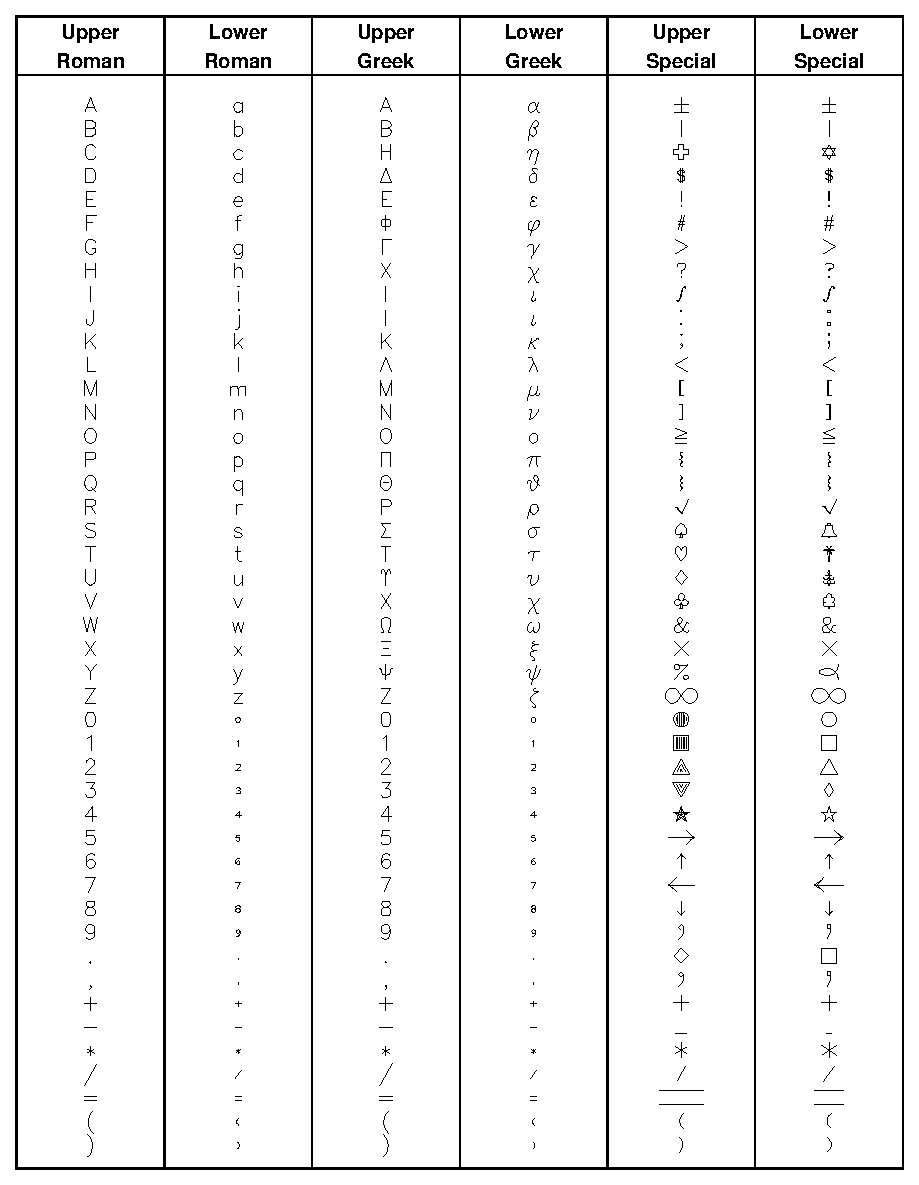
\epsfig{file=softtext.eps}}
\end{center}
\caption{Characters available in \protect\Rind{IGTEXT}}
\label{SOFTTEXT}
\end{figure}
\clearpage 

\Filename{H2Settingattributes}
\section{Setting attributes}
\index{attributes!setting}
\Shubr{IGSET}{(CHNAME,VAL)}
\Action
Routine used to set the value of attributes related to
primitives and/or macroprimitives. 
The first parameter is
the mnemonic name of the parameter, the second is the value to be assigned.
Note that all the
basic primitives attributes can also be set with this routine.
\begin{DLtt}{1234567}
\item[CHNAME] Character variable specifying the name of
the parameter to be set (type {\tt CHARACTER*4}). This is an UPPERCASE
character string.
\item[VAL] {\bf Floating point} value of the parameter (must be specified
as a {\tt REAL} number).\\
A value of {\tt0.0} indicates that the parameter value must
be reset to its default value.
\end{DLtt}

\begin{table}[p]
\index{fill area!interior style}
\index{fill area!style index}
\index{fill area!colour index}
\index{polyline!type}
\index{polyline!width}
\index{polyline!colour index}
\index{polymarker!type}
\index{polymarker!scale factor}
\index{polymarker!colour index}
\index{text!colour index}
\index{text!alignment}
\index{text!character height}
\index{text!angle}
\index{text!font}
\index{text!precision}
\index{text!width}
\index{axis!tick marks size}
\index{axis!labels size}
\index{axis!labels offset}
\index{box!border}
\index{arc!border}
\index{automatic naming of pictures}
\index{colour!map}
\begin{tabularx}{\textwidth}{|c|X|}
\hline
\multicolumn{1}{|c|}{\tt CHNAME} & \multicolumn{1}{c|}{\tt VAL} \\
\hline
'\Sind{FAIS}'     & Fill Area Interior Style (0.,1.,2.,3.). See \Rind{ISFAIS} \\
'\Sind{FASI}'     & Fill Area Style Index. See \Rind{ISFASI}                  \\
'\Sind{LTYP}'     & Line TYPe. See \Rind{ISLN}                                \\
'\Sind{BASL}'     & BAsic Segment Length. See \Rind{ISLN}                     \\
'\Sind{LWID}'     & Line WIDth. See \Rind{ISLWSC}                             \\
'\Sind{MTYP}'     & Marker TYPe. See \Rind{ISMK}                              \\
'\Sind{MSCF}'     & Marker SCale Factor. See \Rind{ISMKSC}                    \\
'\Sind{PLCI}'     & PolyLine Colour Index. See \Rind{ISPLCI}                  \\
'\Sind{PMCI}'     & PolyMarker Colour Index. See \Rind{ISPMCI}                \\
'\Sind{FACI}'     & Fill Area Colour Index. See \Rind{ISFACI}                 \\
'\Sind{TXCI}'     & TeXt Colour Index. See \Rind{ISTXCI}                      \\
'\Sind{TXAL}'     & 10*(horizontal alignment) + (vertical alignment).
                    See \Rind{ISTXAL}                                         \\
'\Sind{CHHE}'     & CHaracter HEight. See \Rind{ISCHH}                        \\
'\Sind{TANG}'     & Text ANGle (used to calculate the Character up vector).
                    See \Rind{ISCHUP}                                         \\
'\Sind{TXFP}'     & 10*(TeXt Font) + (TeXt Precision). See \Rind{ISTXFP}      \\
'\Sind{TMSI}'     & Tick Marks SIze (in \WC). See \Rind{IGAXIS}               \\
'\Sind{LASI}'     & LAbels SIze (in \WC). See \Rind{IGAXIS}                   \\
'\Sind{LAOF}'     & LAbels OFfset. See \Rind{IGAXIS}                          \\
'\Sind{AWLN}'     & Axis Wire LeNght. See \Rind{IGAXIS}                       \\
'\Sind{PASS}'     & Text width (given by number of {\tt PASS}es) of characters
                    drawn by \Rind{IGTEXT}. The width is simulated by shifting
                    the ``pen'' slightly at each pass.                        \\
'\Sind{CSHI}'     & Distance between each shifted drawing of the character
                    (in percentage of the character height)
                    for characters drawn by \Rind{IGTEXT}                     \\
'\Sind{BORD}'     &
\begin{tabular}[t]{ll}
\tt 0.& The border in \Rind{IGBOX}, \Rind{IGFBOX} and \Rind{IGARC}
        is not drawn. \\
\tt 1.& The border in \Rind{IGBOX}, \Rind{IGFBOX} and \Rind{IGARC} is drawn.  \\
\end{tabular}                                                                 \\
'\Sind{PICT}'     & Starting number for the automatic naming of pictures.     \\
'\Sind{AURZ}'     & {\tt 1.} The last current picture is automatically saved on
                    disk when a new picture is created see \Rind{IZPICT}.     \\
'\Sind{*}'        & All attributes are set to their default values.           \\
'\Sind{SHOW}'     & The current value and the default of the parameters
                    controlled by \Rind{IGSET} are displayed.                 \\
'\Sind{BARO}'     & Offset of the left edge of the bar with respect to the left
                    margin of the bin for a bar chart (expressed as a fraction
                    of the bin width). See \Rind{IGHIST}                      \\
'\Sind{BARW}'     & Width of the bar in a bar chart (expressed as a fraction of
                    the bin width). See \Rind{IGHIST}                         \\
'\Sind{NCOL}'     & Number of entry in the COLour map.                        \\
'\Sind{CLIP}'     & Clipping mode: 1.=on 0.=off                               \\
\hline
\multicolumn{1}{|c|}{\tt CHNAME} & \multicolumn{1}{c|}{\tt VAL (For X11 interface only)} \\
\hline
'\Sind{DRMD}'     & Drawing mode: 1.=copy 2.=xor 3.=invert                    \\
'\Sind{SYNC}'     & Synchronise the graphics in X11 1.=yes 0.=no              \\
'\Sind{2BUF}'     & 10*(WKID)+(double buffer mode: 1.=on 0.=off)              \\
\hline
\end{tabularx}

\caption{Overview of \protect\Rind{IGSET} parameters}
\end{table}












